\chapter{Resultados}
\label{chap:resultados}
\section{Introdução}
Para avaliar a eficácia do método de super-resolução bayesiana, 
foi elaborado um teste que simula um sistema de aquisição de imagem,
gerando as imagens de baixa resolução a serem restauradas.
Na sequência, as imagens de baixa resolução foram submetidas ao método de super-resolução como descrito Capítulo \ref{chap:srbayes}.

Este capítulo descreve o processo de implementação e teste do método de super-resolução bayesiana.
A Seção \ref{sec:gerimagens} apresenta o processo que gerou as imagens de teste simulando as transformações aplicadas pelo sistema de aquisição.
A Seção \ref{sec:parestimation} relata como se deu o processo de restauração da imagem de alta resolução a partir do conjunto de imagens de baixa resolução.
Por fim, a Seção \ref{sec:imgestimation} relata o processo de estimação da imagem de alta resolução.


\section{Geração do conjunto de imagens de teste}
\label{sec:gerimagens}

O método de super-resolução Bayesiana foi testado com dois conjuntos de imagens de
baixa resolução geradas artificialmente a partir de duas imagem de alta resolução
distintas.
O modelo de observação exposto na Seção \ref{sec:obsmodel} foi usado para gerar dois conjuntos de 20 imagens de baixa resolução a partir das imagens na Figura \ref{fig:hrimage}.

%As imagens de baixa resolução usadas para testar o método de restauração descrito neste trabalho foram geradas artificialmente a partir de uma única imagem usando o modelo de observação descrito na Seção \ref{sec:obsmodel}.
%Para os testes reportados aqui foi usada a imagem da Figura \ref{fig:hrimage}.
%Usando o modelo de observação, foram geradas 20 imagens de baixa resolução como as da Figura \ref{fig:frames}.
%Para diminuir o custo computacional do processo, a imagem foi convertida para escala de cinza antes da degradação.

\begin{figure}[h]
	\centering
	\caption{\label{fig:hrimage}Imagens de alta resolução utilizadas nos testes.}
	\begin{minipage}[b]{.48\linewidth}
		\centering
		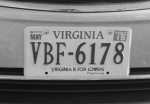
\includegraphics{figures/imtestes.png}
		\subcaption{Exemplar 1: \emph{``Virginia''}.}
	\end{minipage}
	\begin{minipage}[b]{.48\linewidth}
		\centering
		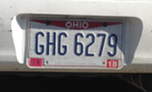
\includegraphics{figures/imteste2s.png}
		\subcaption{Exemplar 2: \emph{``Ohio''}.}
	\end{minipage}
	\legend{Fonte: O autor.}

\end{figure}

Para os testes feitos neste trabalho, ambas as imagens de alta resolução foram
redimensionadas de forma que as dimensões das imagens de baixa resolução são iguais a
$1/4$ das dimensões da imagem HR.  
Na prática, há 16 pontos nas imagens de alta resolução para cada ponto nas imagem de
baixa resolução.

Sobre os parâmetros de degradação escolhidos. A largura da função de espalhamento de ponto ($\gamma$) escolhida foi 2.
Para cada imagem, o ângulo de rotação foi escolhido aleatoriamente de uma distribuição uniforme entre $-4$ e $4$ graus.
A mesma seleção aleatória foi feita para o deslocamento linear da imagem; a quantidade de pontos de deslocamento foi retirada de uma distribuição uniforme e contínua entre $-2$ e $2$ em cada um dos eixos.
A Tabela \ref{tab:resumoParametros} resume os parâmetros utilizados na degradação das imagens.

% ISSUE: Falar dimensões das imagens HR.

\begin{figure}[H]
	\centering
	\caption{\label{fig:frames}
	Conjunto das imagens geradas a partir do Exemplar 1: \emph{"Virginia"}. A diferença sutil entre as imagens é causada pelas transformações de deslocamento e rotação.
	As dimensões de cada imagem são de $38 \times 26$.}
	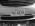
\includegraphics{figures/degradedImg/result-0.png}
	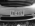
\includegraphics{figures/degradedImg/result-1.png}
	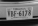
\includegraphics{figures/degradedImg/result-2.png}
	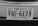
\includegraphics{figures/degradedImg/result-3.png}
	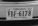
\includegraphics{figures/degradedImg/result-4.png}
	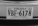
\includegraphics{figures/degradedImg/result-5.png}
	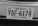
\includegraphics{figures/degradedImg/result-6.png}
	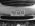
\includegraphics{figures/degradedImg/result-7.png}
	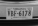
\includegraphics{figures/degradedImg/result-8.png}
	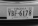
\includegraphics{figures/degradedImg/result-9.png} 

	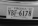
\includegraphics{figures/degradedImg/result-10.png}
	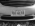
\includegraphics{figures/degradedImg/result-11.png}
	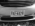
\includegraphics{figures/degradedImg/result-12.png}
	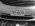
\includegraphics{figures/degradedImg/result-13.png}
	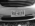
\includegraphics{figures/degradedImg/result-14.png}
	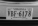
\includegraphics{figures/degradedImg/result-15.png}
	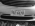
\includegraphics{figures/degradedImg/result-16.png}
	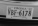
\includegraphics{figures/degradedImg/result-17.png}
	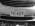
\includegraphics{figures/degradedImg/result-18.png}
	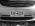
\includegraphics{figures/degradedImg/result-19.png}
	\legend{Fonte: O autor.}
	
\end{figure}
\begin{figure}[H]
	\centering
	\caption{ Conjunto das imagens geradas a partir da do Exemplar 2: \emph{"Ohio"}.
	As dimensões de cada imagem são de $38 \times 23$.}
	\label{fig:frames2}
	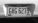
\includegraphics{figures/degradedImg2/result-0.png}
	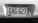
\includegraphics{figures/degradedImg2/result-1.png}
	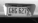
\includegraphics{figures/degradedImg2/result-2.png}
	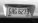
\includegraphics{figures/degradedImg2/result-3.png}
	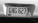
\includegraphics{figures/degradedImg2/result-4.png}
	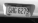
\includegraphics{figures/degradedImg2/result-5.png}
	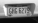
\includegraphics{figures/degradedImg2/result-6.png}
	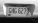
\includegraphics{figures/degradedImg2/result-7.png}
	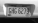
\includegraphics{figures/degradedImg2/result-8.png}
	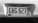
\includegraphics{figures/degradedImg2/result-9.png} 

	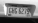
\includegraphics{figures/degradedImg2/result-10.png}
	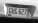
\includegraphics{figures/degradedImg2/result-11.png}
	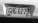
\includegraphics{figures/degradedImg2/result-12.png}
	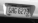
\includegraphics{figures/degradedImg2/result-13.png}
	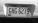
\includegraphics{figures/degradedImg2/result-14.png}
	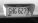
\includegraphics{figures/degradedImg2/result-15.png}
	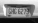
\includegraphics{figures/degradedImg2/result-16.png}
	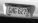
\includegraphics{figures/degradedImg2/result-17.png}
	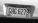
\includegraphics{figures/degradedImg2/result-18.png}
	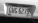
\includegraphics{figures/degradedImg2/result-19.png}
	\legend{Fonte: O autor.}
	
\end{figure}

\begin{table}[h]
	\centering
	\caption{Parâmetros de degradação usados para gerar o conjunto de imagens de teste.}
	\label{tab:resumoParametros}
	\begin{tabular}{r | l}
		Ângulos de rotação ($\theta_k$) & $ \sim \mathcal{U}(-4, 4)$ \\ \hline
		Deslocamento ($\mathbf{s}_k$)& $\sim \mathcal{U}(-2,2)$\\ \hline
		Largura da PSF ($\gamma$) & 2 \\ 

	\end{tabular}
	\legend{Fonte: O autor.}
\end{table}

O processo de geração das imagens de baixa resolução foi todo desenvolvido usando a linguagem Python,
beneficiando-se dos módulos Numpy e Pillow.
Os parâmetros de degradação bem como as dimensões da imagem original foram salvas em arquivos de valores separados por vírgula (csv) junto com as imagens geradas.
Esses valores foram usados para avaliar quantitativamente a efetividade do algorítimo de
otimização em inferir os valores corretos dos parâmetros.

\section{Estimação dos parâmetros de degradação}
\label{sec:parestimation}
A primeira etapa no processo de restauração da imagem é estimar os parâmetros que definiram as transformações que degradaram a imagem durante o processo simulado de captura. Como já elucidado no Capítulo \ref{chap:srbayes}, encontrar os valores dos parâmetros de degradação é um problema de otimização.
Teoricamente, os valores verdadeiros de $\mathbf{s}_k$, $\theta_k$ e $\gamma$ são os que maximizam a função de verosimilhança em (\ref{eq:parameter}).

% ISSUE: Pesquisar sobre o conceito de otimização.

O artigo no qual este trabalho se baseia relata que o método de otimização usado
para estimar tanto os parâmetros de degradação quanto da imagem foi o de gradientes
conjugados \cite{tipping2003bayesian}.
Como o método de super-resolução deste trabalho foi todo escrito em Python,
não foi possível utilizar o mesmo método de implementação empregado no artigo.
Em vez disso, foi usado um Método de Newton Truncado \cite{nocedal1999optimization} presente no módulo \emph{Scipy}.

% SUGGESTION: Falar mais sobre o algorítimo de otimização Método de Newton Truncado. Talvez em um apêndice.

O processo de otimização dos parâmetros se deu da seguinte forma:
Os parâmetros de rotação e deslocamento foram definidos como zero;
a largura da função de espalhamento de ponto inicial foi 4.
Então, a otimização dos parâmetros se deu em três partes:
\begin{enumerate}
	\item Na primeira, somente os valores de deslocamento são otimizados enquanto os valores dos ângulos de rotação permanecem fixos.
	\item Na segunda, é realizada a otimização dos ângulos de rotação junto com os deslocamentos lineares.
	\item Em uma terceira parte, a largura da função de espalhamento de ponto ($\gamma$) é otimizada concomitantemente com os demais parâmetros.
\end{enumerate}

Essa abordagem é usada no artigo original e os testes realizados para este trabalho
constataram que a otimização dos parâmetros de deslocamento se aproxima mais rápido da
solução correta quando esses valores são estimados isoladamente.
A estimação dos ângulos também funciona melhor quando os valores de deslocamento já estão
otimizados.


Um fato que merece destaque é o de que, como a função em (\ref{eq:parameter}) não é uma
função vetorial do tipo $ f(\mathbf{x}) : \mathbb{R}^n \to \mathbb{R}^1 $, não foi 
possível passá-la diretamente ao método de otimização.
Por isso, foi necessário empacotar a função de forma que ela recebesse os parâmetros de
entrada ($\mathbf{s}_k$, $\theta_k$ e $\gamma$) reorganizados na forma de um único
vetor e retornasse somente um escalar na saída.
Isso também implicou na exigência de calcular numericamente o gradiente da função,
necessário na execução do método de otimização.

O método de super resolução Bayesiana faz uso de matrizes esparsas como $\mathbf{Z}_x$ e $\mathbf{\Sigma}$ no seu modelo matemático que representam uma grande custo computacional em memória e tempo de processamento.
Para reduzir esse custo, foi usada somente uma janela de $7 \times 7$ pontos do centro de
cada imagem de baixa resolução para estimar os parâmetros de degradação.
Neste caso, a janela de cada imagem foi empregada como se fosse a própria
imagem de baixa resolução.

A função de otimização com algorítimo de Newton truncado presente na biblioteca
\emph{Scipy} permite que sejam definidos limites para restringir o intervalo de busca
no espaço vetorial onde a estimação é feita.
Isso é especialmente útil, pois permite usarmos um conhecimento a priori acerca dos
parâmetros para impedir que a otimização retorne resultados inviáveis que, por ventura,
tenham um alto valor de verossimilhança.
Os limites definidos para os parâmetros foram de -4 a 4 no caso dos ângulos de rotação,
-2 a 2 para ambas as direções dos deslocamentos e 1 a 7 para a largura da função de
espalhamento de ponto.

Para reduzir o tempo gasto na execução da otimização dos parâmetros, o número máximo de avaliações da função de verossimilhança por etapa foi restringido.
Na primeira etapa, o número máximo de avaliações da função de verossimilhança foi de 70.
Em ambas as etapa subsequentes este limite foi de 50 avaliações.
Esses limites não interferem na qualidade do resultado pois, mesmo que eles sejam bem maiores, o valor das avaliações da função estabiliza após poucas iterações.

% SUGGESTION: Talvez seja melhor usar gradiente em vez de número de avaliações como critério de parada

Durante a execução do Método de Newton Truncado, foram registrados o valor da função de verossimilhança e o erro da solução atual ao fim de cada iteração.
O erro calculado é igual $\|\mathbf{c}_{atual} - \mathbf{c}_{real}\|$ onde
$\mathbf{c}_{atual}$ é o vetor com os parâmetros obtidos ao fim da iteração e
$\mathbf{c}_{real}$ é o vetor com os parâmetros verdadeiros usado para a comparação.
Os resultados desta análise são ilustrados na Figura \ref{fig:progression_plots}.

\begin{figure}
	\centering
	\caption{Progressão dos valores da avaliação da função de verossimilhança e do erro dos parâmetros estimados a cada iteração do algorítimo de otimização.}
	\label{fig:progression_plots}
	\begin{minipage}[b]{.99\linewidth}
		\centering
		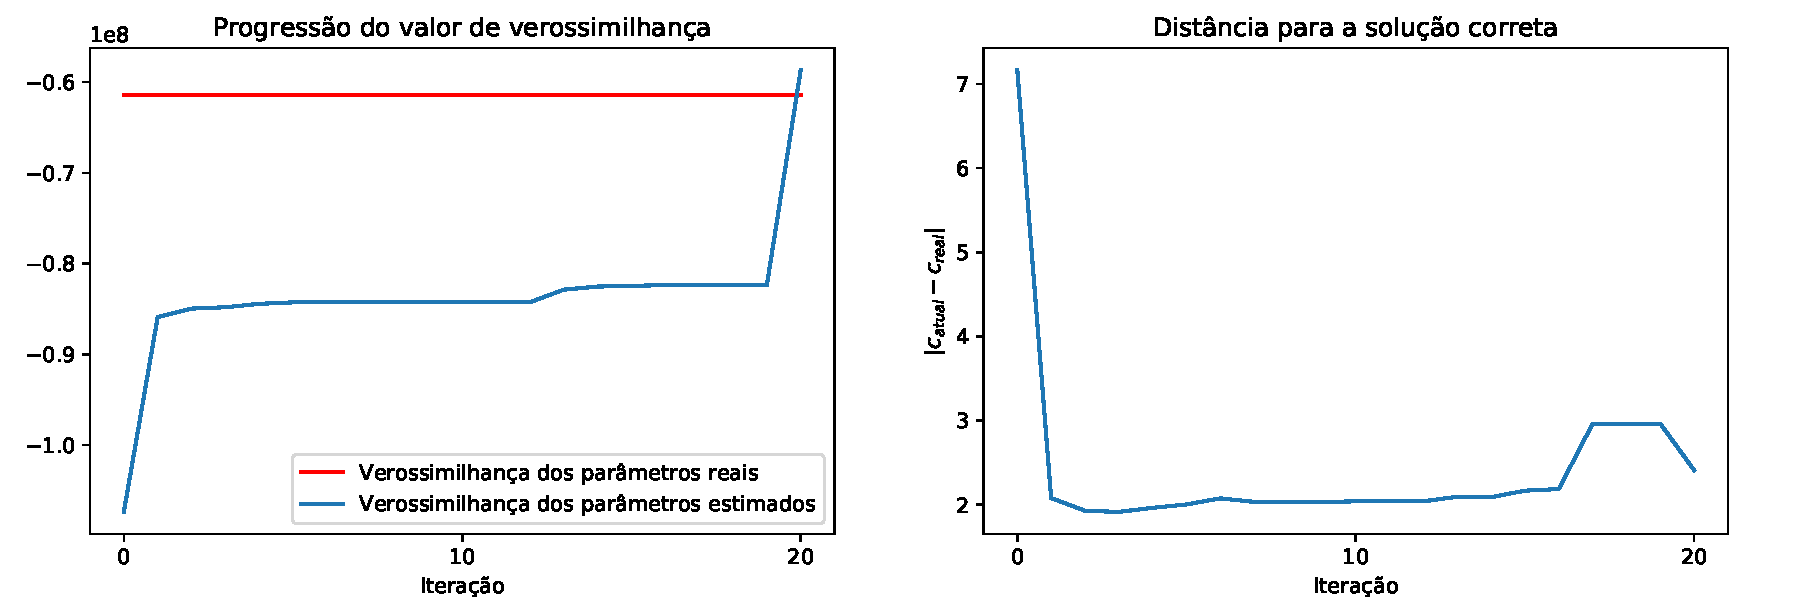
\includegraphics[width=0.90\textwidth]{./figures/results_figures/progression_plot.pdf}
		\subcaption{Resultados obtidos com a estimação do Exemplar 1: \emph{``Virginia''}}
	\end{minipage}

	\begin{minipage}[b]{.99\linewidth}
		\centering
		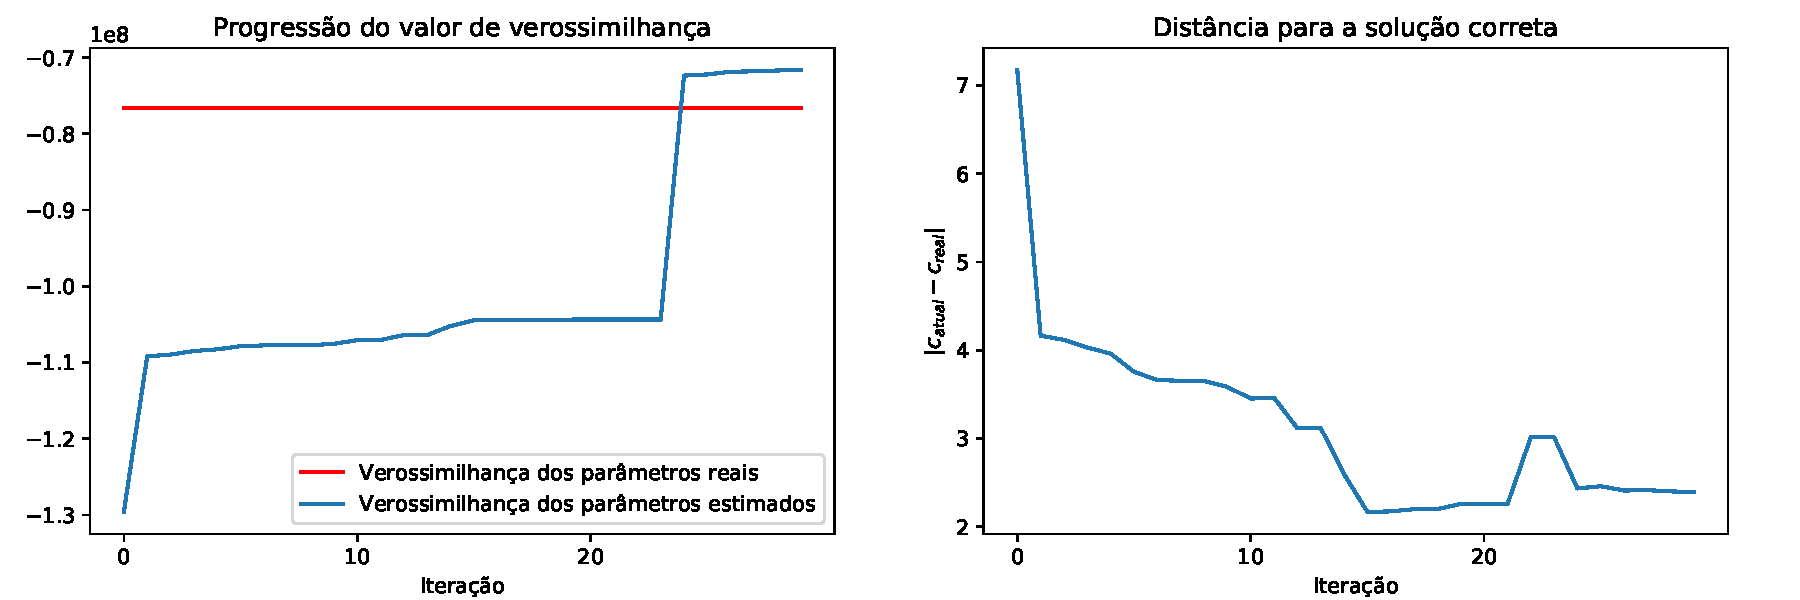
\includegraphics[width=0.90\textwidth]{./figures/results_figures/progression_plot2.pdf}
		\subcaption{Resultados obtidos com a estimação do Exemplar 2: \emph{``Ohio''}}
	\end{minipage}
	\legend{Fonte: O autor}
\end{figure}
% SUGGESTION: Escrever pseudocódigo do empacotamento da função de verossimilhança dos parâmetros.

Ao final da execução do algorítimo de otimização, os os valores obtidos foram
colhidos e comparados com os parâmetros de transformação reais. O resultado dessa
comparação está retratado na Figura \ref{fig:comparisson_plots}. 

% SUGGESTION: Mostrar o gráfico da verossimilhança para os valores de gamma.

A estimativa da largura da função de espalhamento de ponto foi de 1 para ambas as imagens testadas;
o que indica que o método não foi eficaz para estimar com precisão o valor de $\gamma$.


\begin{figure}
	\centering
	\caption{Comparação dos resultados obtidos ao final da execução do algorítimo de otimização com os parâmetros verdadeiros.}
	\label{fig:comparisson_plots}
	\begin{minipage}[b]{.99\linewidth}
		\centering
		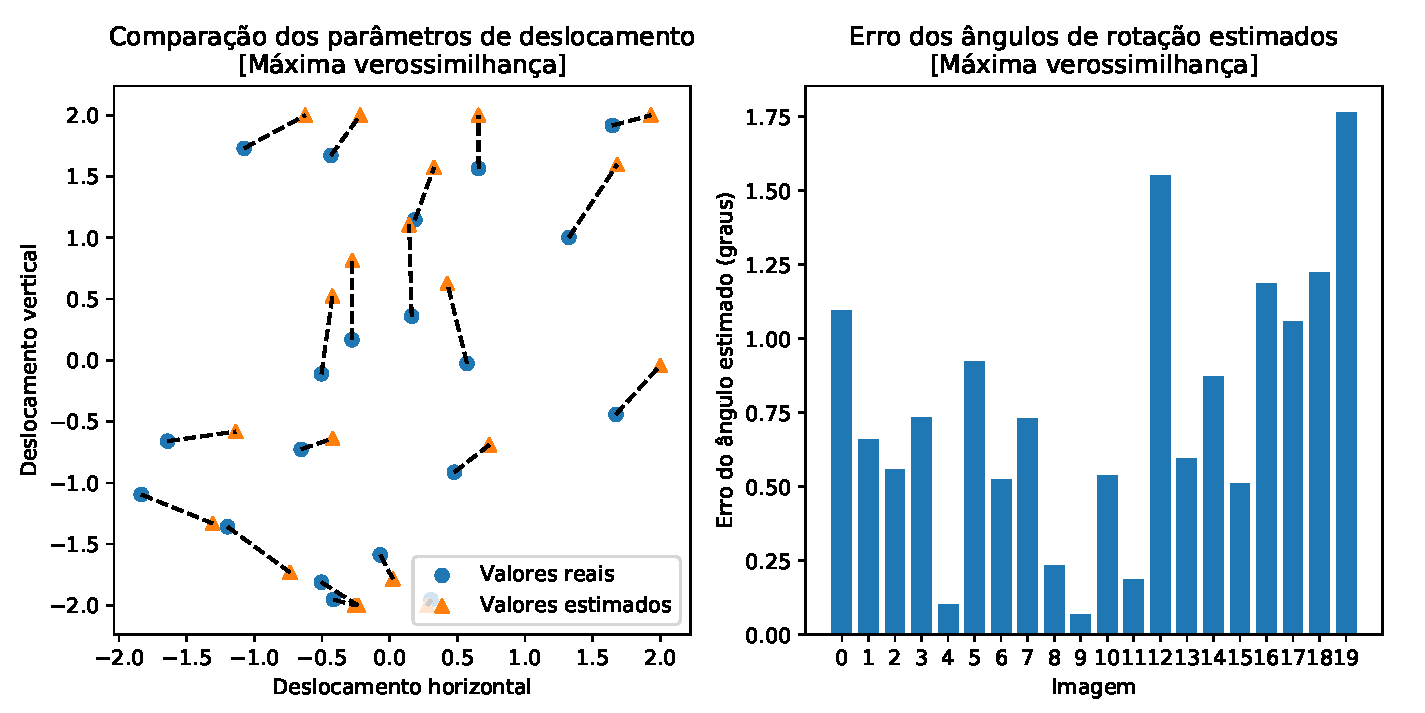
\includegraphics[width=0.8\textwidth]{./figures/results_figures/comparisson_plot.pdf}
		\subcaption{Resultados obtidos com a estimação do Exemplar 1: \emph{``Virginia''}}
	\end{minipage}

	\begin{minipage}[b]{.99\linewidth}
		\centering
		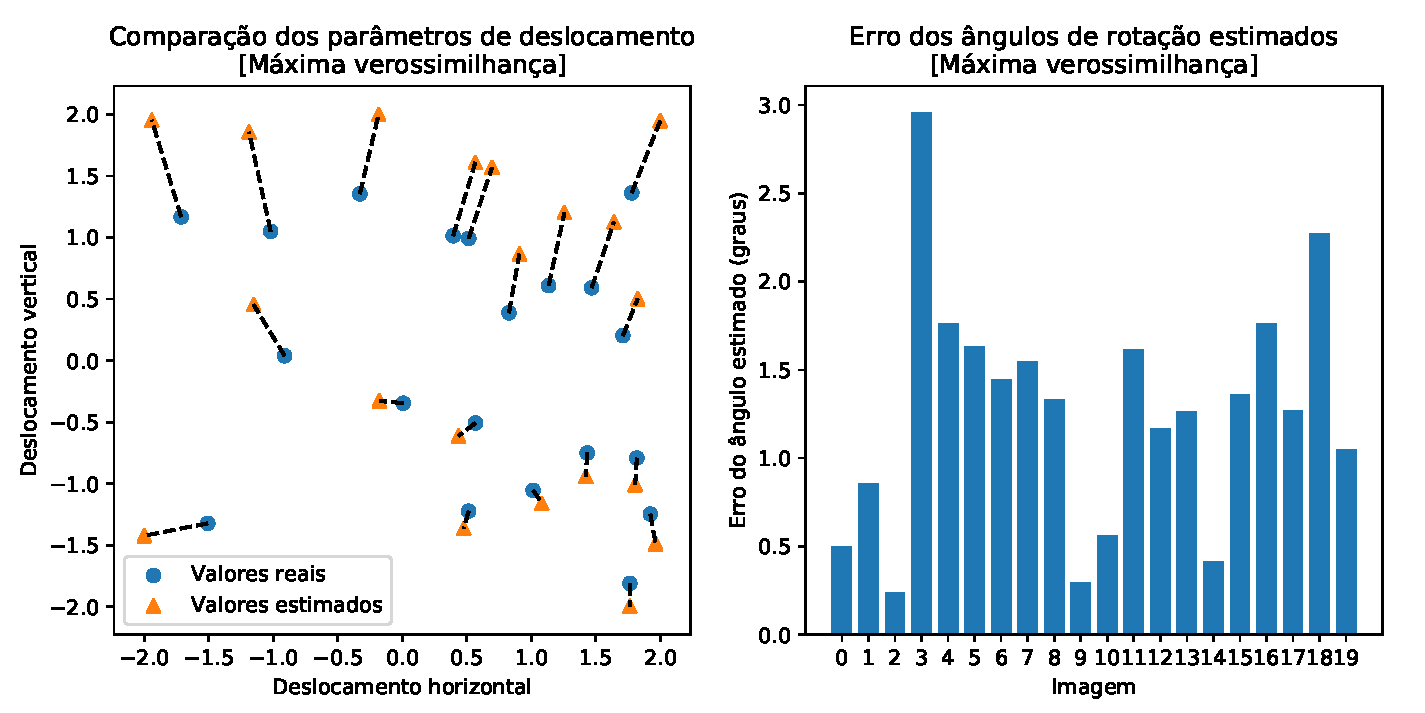
\includegraphics[width=0.8\textwidth]{./figures/results_figures/comparisson_plot2.pdf}
		\subcaption{Resultados obtidos com a estimação do Exemplar 2: \emph{``Ohio''}}
		
	\end{minipage}
	\legend{Fonte: O autor}
\end{figure} 

\begin{table}[H]
	\caption{Tempos de execução e número de iterações no algorítimo de Newton truncado para cada um dos exemplares.}
	\label{tab:temposexec}
	\begin{tabular}{r || l | l}
		 & Exemplar 1: \emph{"Virginia"} & Exemplar 2: \emph{"Ohio"} \\ \hline
		Tempo de execução & 31 minutos e 39 segundos & 37 minutos e 23 segundos \\ \hline
		Número de iterações & 18 & 27
	\end{tabular}
	\legend{Fonte: O autor}
\end{table}

\clearpage
\section{Estimação da imagem de alta resolução}
\label{sec:imgestimation}
Após a estimação dos parâmetros de degradação, os valores otimizados deve ser passados para a função de verossimilhança da imagem em (\ref{eq:imageLikelihood}) para que seja estimada a imagem de alta resolução em si.

O algorítimo de Newton truncado também foi usado para estimar a imagem de acordo com as imagens observadas e os parâmetros de degradação.
Ao contrário do que aconteceu na etapa anterior, não foi necessário calcular o gradiente da função numericamente para esta etapa.
Como a função de verossimilhança em (\ref{eq:imageLikelihood}) é uma função vetorial do tipo $ f(\mathbf{x}) : \mathbb{R}^n \to \mathbb{R}^1$, então foi relativamente simples calcular seu gradiente mostrado na Equação (\ref{eq:imageLikelihood_gradient}).

A possibilidade de se calcular o gradiente da função analiticamente em vez de numericamente teve como consequência um ganho considerável de desempenho com redução no tempo de execução do algorítimo.
Esse ganho de desempenho foi bastante importante devido à quantidade de dados a serem estimados.
Para uma imagem com dimensões de $150 \times 104$, o vetor $\mathbf{x}$ chega a ter 15600 elementos.

A função de verossimilhança da imagem depende da inversa da matriz de covariância $\mathbf{Z}_x^{-1}$ e de $\log{|\mathbf{Z}_x|}$.
Como a matriz de covariância tem muitos elementos e é sempre a mesma para imagens de dimensões iguais, esse valores foram salvos em disco para economizar tempo em vários testes sucessivos com a mesma imagem.

Ao final da execução do algorítimo de otimização, as imagens obtidas foram as imagens de
baixo contraste retratadas nas Figuras \ref{fig:result_histograms2_output} e
\ref{fig:result_histograms1_output}.
Para revelar os resultados foi necessário equalizar os histogramas das imagens obtidas,
o que resultou nas imagens retratadas nas Figuras \ref{fig:result_histograms2_equalized}
e \ref{fig:result_histograms1_equalized}.

\begin{figure}
	\centering
	\caption{Resultados obtidos com a otimização do Exemplar 1: \emph{"Virginia"}}
	\label{fig:result_histograms2}
	\begin{minipage}[b]{.99\linewidth}
		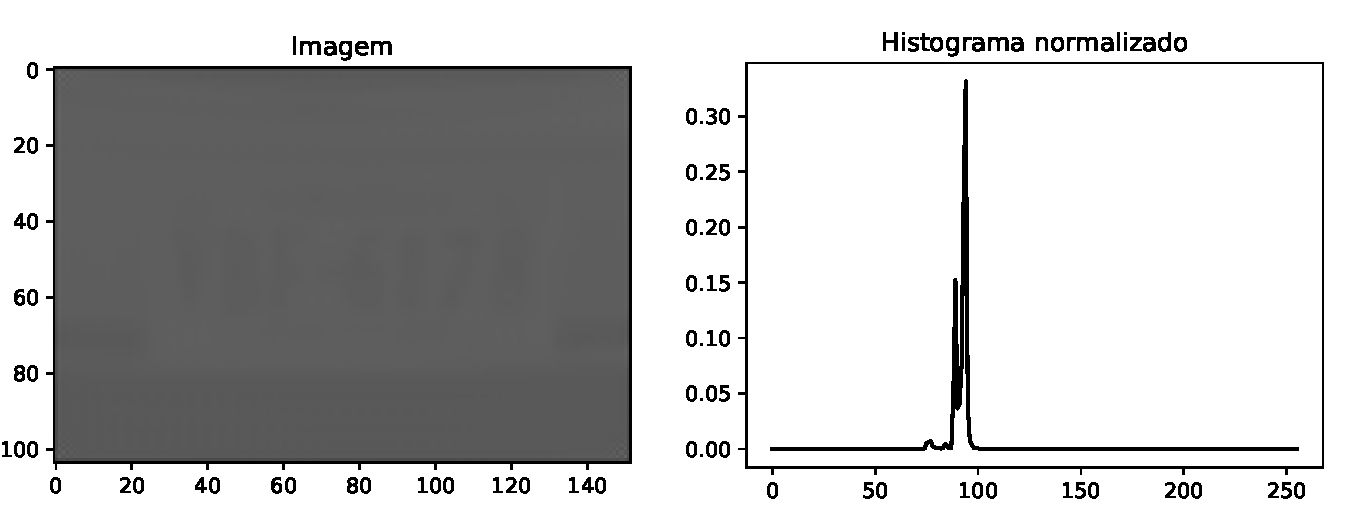
\includegraphics[width = 0.9\textwidth]{./figures/results_figures/histograma3.pdf}
		\subcaption{Imagem resultante do processo de otimização juto com seu histograma.}
		\label{fig:result_histograms2_output}
	\end{minipage}	

	\begin{minipage}[b]{.99\linewidth}
		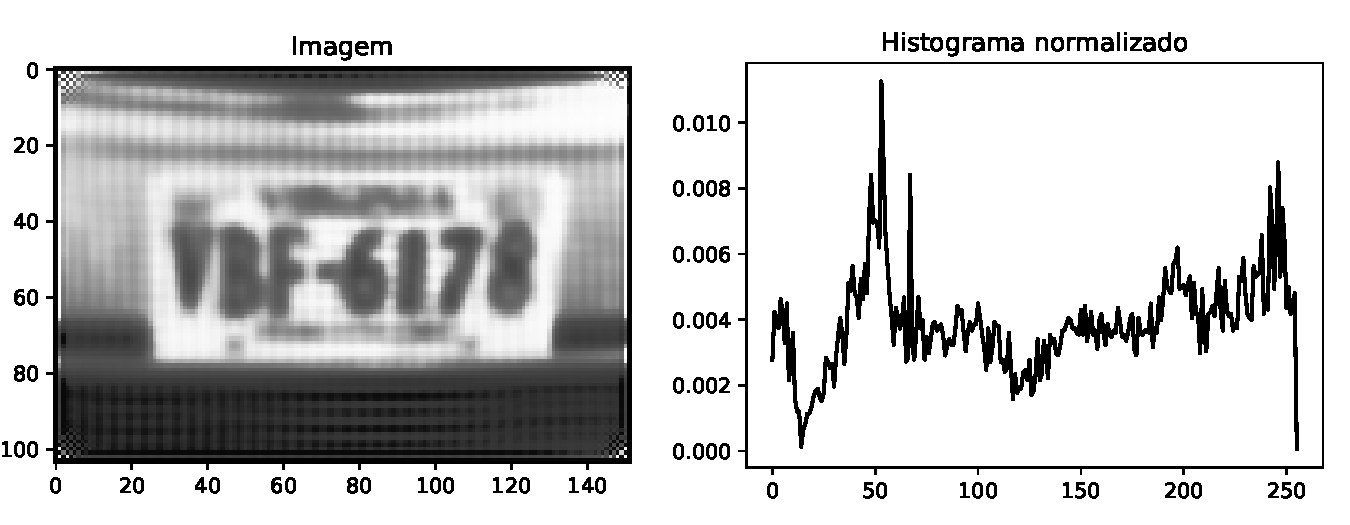
\includegraphics[width = 0.9\textwidth]{./figures/results_figures/histograma4.pdf}
		\subcaption{Imagem resultante após equalização de histograma.}
		\label{fig:result_histograms2_equalized}
	\end{minipage}	
	\legend{Fonte: O autor.}
	
\end{figure}

\begin{figure}
	\centering
	\caption{Resultados obtidos com a otimização do Exemplar 2: \emph{"Ohio"}}
	\label{fig:result_histograms1}
	\begin{minipage}[b]{.99\linewidth}
		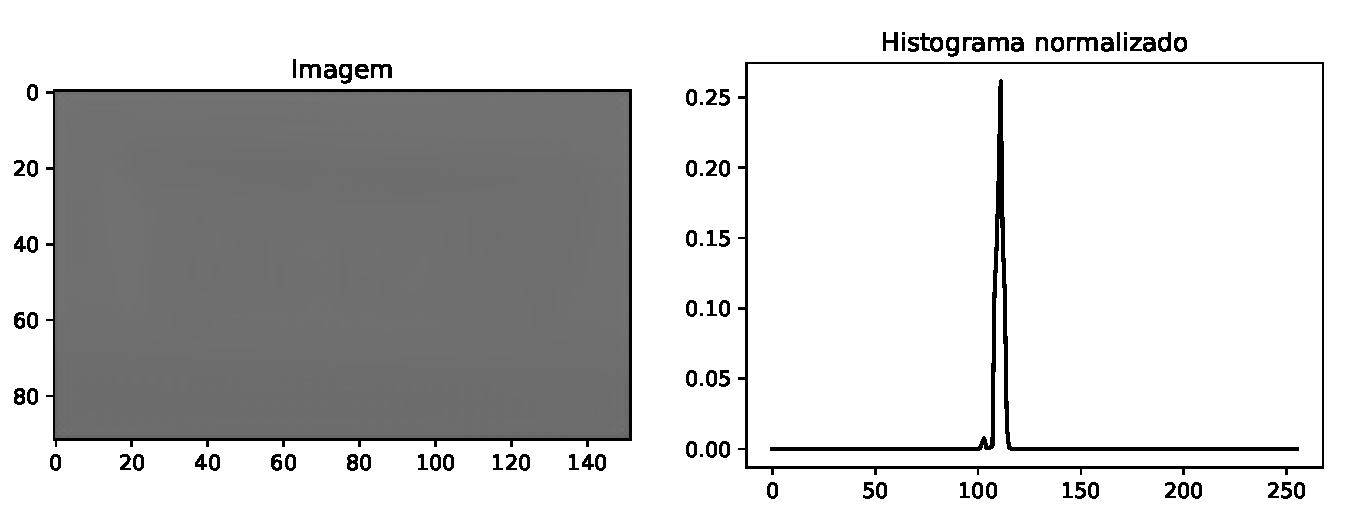
\includegraphics[width = 0.9\textwidth]{./figures/results_figures/histograma2.pdf}
		\subcaption{Imagem resultante do processo de otimização juto com seu histograma.}
		\label{fig:result_histograms1_output}
	\end{minipage}	

	\begin{minipage}[b]{.99\linewidth}
		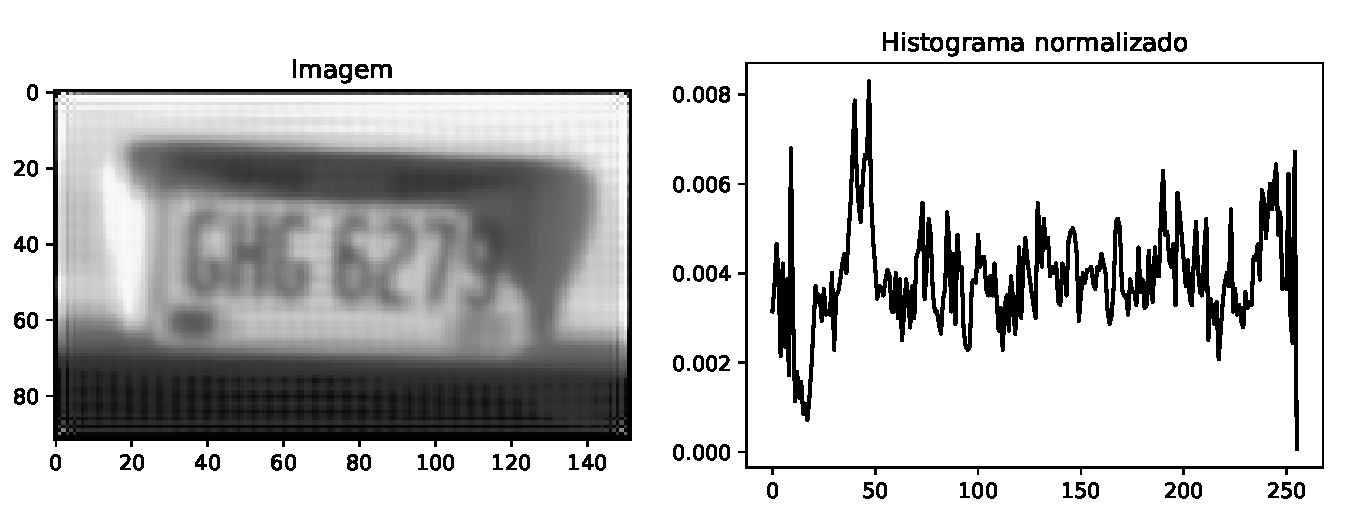
\includegraphics[width = 0.9\textwidth]{./figures/results_figures/histograma1.pdf}
		\subcaption{Imagem resultante após equalização de histograma.}
		\label{fig:result_histograms1_equalized}
	\end{minipage}	
	\legend{Fonte: O autor.}
	
\end{figure}

A Figura \ref{fig:results_compare} compara as imagens de baixa resolução, redimensionada usando usando interpolação bicúbica (um método presente nos principais softwares de edição de imagens), restaurada usando o método de Super-resolução bayesiana e a imagem de alta resolução original.

\begin{figure}
	\centering
	\caption{Comparação do resultado obtido através do método de super-resolução Bayesiana com a simples interpolação da imagem.}
	\label{fig:results_compare}
	\includegraphics[width = 0.95\textwidth]{./figures/results_figures/result_compare.pdf}
	\legend{Fonte: O autor.}
\end{figure}

A Tabela \ref{tab:temposexec2} mostra os tempos de execução, número de iterações e de avaliações da função da execução do Método de Newton Truncado para cada exemplar.

\begin{table}
	\caption{Tempos de execução e número de iterações no algorítimo de Newton truncado para cada um dos exemplares.}
	\label{tab:temposexec2}
	\begin{tabular}{r || l | l}
		 & Exemplar 1: \emph{"Virginia"} & Exemplar 2: \emph{"Ohio"} \\ \hline
		Tempo de execução & 4 minutos e 24 segundos & 7 minutos e 24 segundos\\ \hline
		Número de iterações & 2 & 2 \\ \hline
		Número de avaliações da função & 90 & 89
	\end{tabular}
	\legend{Fonte: O autor}
\end{table}


